\section{approach}
\label{sec:approach}
In this section, we first formulate the just-in-time defect prediction and provide an overview of our framework. We then describe the details of each part inside the framework. Finally, we present an algorithm for learning effective settings of our model's parameters. 
\subsection{Framework Overview}
\label{sec:overview}

\begin{figure}
\center
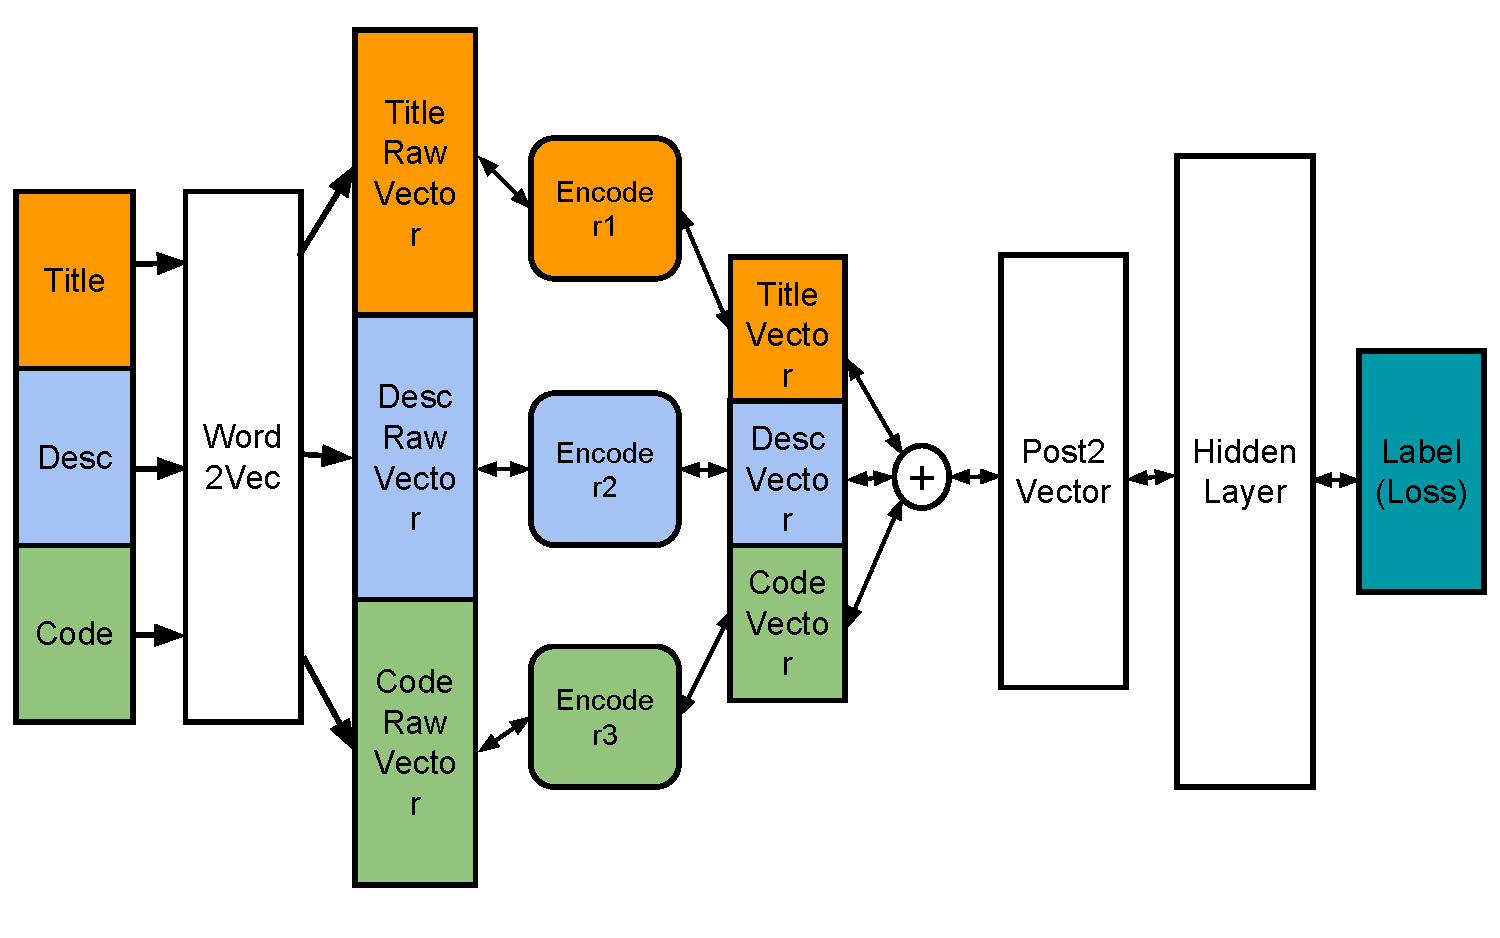
\includegraphics[scale=0.36]{figs/framework.pdf}
\caption{The general framework of just-in-time defect prediction model.}
\label{fig:overview}
\end{figure}

The goal of the just-in-time defect prediction model is to automatically label a commit change as bug or clean to help developers better focus on their efforts on assuring software quality. We consider the just-in-time defect prediction problem as a learning task to construct prediction function: $f:
\mathcal{X} \longmapsto \mathcal{Y}$, where $y_i \in \mathcal{Y} = \{0, 1\}$ indicates whether a commit change $x_i \in \mathcal{X}$ contains a buggy code or clean. The prediction function $f$ can be learned by minimizing the following objective function:
\begin{equation}
\underset{f}{min} \sum_{i}\mathcal{L}(f(x_i), y_i) + \lambda\Omega(f)
\end{equation}
where $\mathcal{L}(.)$ is the empirical loss function measuring the difference between the predicted and the output label, $\Omega(f)$ is a regularization function to prevent the over fitting problem, and $\lambda$ the trade-off between $\mathcal{L}(.)$ and $\Omega(f)$. Figure~\ref{fig:overview} illustrates the overview framework of the just-in-time defect prediction model. The model consists of four parts: input layer, feature extraction layer, feature combination layer, and the output layer.  